
\subsubsection{OpenAppSec}
Während des Freigabeprozesses äußerte der Mandant, dass der konkrete Nutzen von OpenAppSec innerhalb seines Setups für ihn nicht eindeutig nachvollziehbar sei. Er bat daher um eine Erläuterung der Einsatzzwecke von OpenAppSec, seiner Funktionsweise, der Rolle von \ac{ML} im System und den konkreten Beitrag zur Angriffserkennung und -abwehr.

OpenAppSec ist eine Open-Source-Firewall für Web- und \ac{API}-Sicherheit (auch \ac{WAF} genannt), die auf Contextual Machine Learning basiert \cite{openappsec_tech}. Die \acs{WAF} wird nicht als Ersatz für Tor oder sonstige notwendige Sicherheitskonfiguration eingesetzt, sondern soll als zusätzliche Schutzschicht vor den Weboberflächen und \acs{API} der eingesetzten Dienste fungieren. Dieser Schutz ist besonders relevant, da das geplante System zahlreiche über \acs{HTTP}/S erreichbare Dienste enthält (z.B.  Authelia, Vaultwarden, Home Assistant, Paperless-ngx, Immich, Jellyfin, Grafana). Auch wenn die Dienste ausschließlich über Tor Onion Services erreichbar gemacht werden, bleiben sie trotzdem Webanwendungen mit Requests, Parametern, Headern, Logins, Uploads und teilweise \acs{API}. Tor schützt vor allem die Erreichbarkeit, die Standortdaten und die Transportebene \cite{tor_onion_services}. Er analysiert jedoch nicht, ob ein eingehender \acs{HTTP}-Request selbst bösartig ist.

Der Einsatz von Tor Onion Services ist laut dem Mandanten zwingend umzusetzen, da er weltweit aus potenziell überwachten oder eingeschränkten Netzen auf seine Dienste zugreifen können soll, ohne dabei unnötige Metadaten an lokale Provider preiszugeben. Er fordert außerdem ausdrücklich eine kompromisslose Absicherung auf Software- und Netzwerkebene sowie die Berücksichtigung realistischer Remote-Angriffe, darunter Malware, Phishing, Brute Force und Supply-Chain-Angriffe. OpenAppSec dient hier der Absicherung der Anwendungsebene. Damit ergänzt OpenAppSec den Tor-basierten Zugriff sinnvoll, denn während Tor die öffentliche Sichtbarkeit des Mandanten schützt, prüft die \acl{WAF} die Web- und \ac{API}-Requests. \cite{tor_onion_services, owasp_waf}

Trotz des eingesetzten Tor Browsers, ist eine \ac{WAF} weiterhin sinnvoll, da Tor nicht vor Angriffen schützt, die innerhalb legitimer \acs{HTTP}-Requests stattfinden. Eine \ac{WAF} bwfindet sich deshalb vor den Anwendungen und bewertet den Inhalt der Requests, bevor diese die eigentlichen Anwendungen erreichen. Nach der Einordnung von \ac{OWASP}, schützen \acs{WAF}s spezifisch Webanwendungen und können als Reverse Proxy vor eine Anwendung geschaltet werden, um Angriffe wie \ac{XSS} oder \ac{SQL}-Injection zu erkennen und zu blockieren. \cite{owasp_waf} \newline \newline
Die \acs{WAF} ist darauf ausgelegt, Angriffe gemäß der \acs{OWASP} Top 10 sowie unbekannte bzw. Zero-Day-Angriffe zu erkennen und abzuwehren \cite{openappsec_security_practices}. Auch wenn Zero-Day-Angriffe laut des Mandanten nicht im Scope sind und damit nicht zum Threat Model gehören, ist die Fähigkeit zur Erkennung unbekannter Angriffsmuster ein zusätzlicher Pluspunkt. Genau hier ist ein Schutz der Anwendungen sinnvoll, weil auch ein nicht direkt exponierter Dienst über fehlerhafte Eingaben, kompromittierte Clients oder später entdeckte Schwachstellen angegriffen werden kann. \newline \newline
Die Funktion des \acl{ML}s ist die Erkennung und Prävention von Web- und \acs{API}-Angriffen im laufenden \acs{HTTP}/S-Verkehr. Der Unterschied zu einer klassischen signaturbasierten \ac{WAF} liegt darin, dass OpenAppSec Requests nicht nur mit bekannten festen Mustern vergleicht, sondern den Request mehrstufig normalisiert, auf Angriffshinweise untersucht und anschließend im Kontext der konkreten Anwendung bewertet. Dies erfolgt laut OpenAppSec in drei Phasen: 
\begin{enumerate}
    \item Zunächst werden alle relevanten Teile eines \acs{HTTP}-Requests dekodiert und normalisiert, darunter z. B. \ac{URL}, Header sowie Payloads.
    \item Anschließend wird nach Hinweisen gesucht, die aus trainierten Mustern bekannter Angriffe abgeleitet werden können.
    \item Abschließend findet eine kontextuelle Bewertung des Requests anhand der konkreten Umgebung, des Nutzers, der \acs{URL} und weiterer Faktoren statt und es wird daraus ein Confidence Score berechnet. Überschreitet dieser Score einen Schwellenwert, wird der Request von der Firewall blockiert (siehe Abbildung \ref{fig1}). \cite{openappsec_tech}
\end{enumerate}  

\begin{figure}[H]
    \centering
    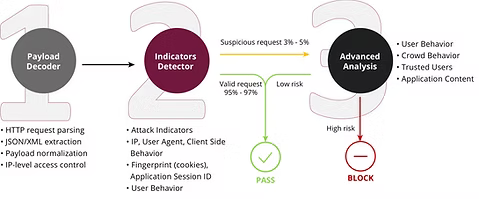
\includegraphics[width=0.8\textwidth]{Abbildungen/OpenAppSecML.png}
    \caption{Schematische Darstellung des mehrstufigen Analyseprozesses von OpenAppSec zur Bewertung von \acs{HTTP}-Requests \cite{openappsec_tech}}
    \label{fig1}
\end{figure}

\paragraph{Was ist Contextual Machine Learning?}

Wie bereits zuvor erwähnt, kombiniert die \acs{WAF} von OpenAppSec die  klassische signaturbasierte Angriffserkennung mit einem auf \acl{ML} basierenden, kontextualisierten Analyseansatz. Anstatt ausschließlich bekannte Signaturen oder feste Muster im \acs{HTTP}/S-Verkehr zu prüfen, werden Requests in Relation zum erwarteten Verhalten der konkreten Anwendung bewertet. Ein identischer Payload kann somit, je nach Kontext, unterschiedlich eingestuft werden. Ein Suchparameter eines Services, ein Login in Authelia oder ein Upload in Paperless-ngx stellen beispielsweise unterschiedliche Kontexte dar und sollten daher nicht mit identischen starren Regeln bewertet werden. \cite{openappsec_tech}

Technisch besteht das \ac{ML}-Konzept aus zwei unterschiedlichen Ebenen. Einerseits nutzt OpenAppSec ein überwachtes Modell, das offline anhand verschiedener Requests trainiert wurde und typische Angriffsmuster erkennt. Andererseits wird ein unüberwachtes Modell in dem eigenen System aufgebaut, das das normale Verhalten des Systems erlernt. Dadurch kann die \ac{WAF} nicht nur bekannte Angriffsmuster wiedererkennen, sondern auch auffällige Abweichungen vom erwarteten Verhalten aufdecken. Dies ist der zentrale Vorteil der anomaliebasierten Erkennung bzw. des Contextual Machine Learnings. Die Entscheidung basiert nicht nur auf einzelnen, bereits bekannten Signaturen, sondern auf einer Gesamtbewertung aus Payload, Angriffshinweisen und Anwendungskontext.\cite{openappsec_github, openappsec_tech}

Dieser Ansatz ist nicht nur ein Hersteller-Claim, sondern wird auch durch aktuelle Forschung zu \ac{ML}-basierten \acs{WAF} grundsätzlich gestützt. Eine 2025 veröffentlichte Studie zu \ac{ML}-basierten \acs{WAF} beschreibt, dass solche Systeme insbesondere für die Erkennung von Injection-Angriffen wie \ac{XSS}, \ac{SQL}-Injection, OS Command Injection und Local File Inclusion eingesetzt werden können. In der dort beschriebenen Evaluation erreichte die \ac{WAF} bei Testungen eine Accuracy von 93,27\% und einen F1-Score von 93,13\%. Die Studie stützt damit die technische Grundannahme, dass \ac{ML}-basierte \acp{WAF} gegenüber rein regelbasierten Ansätzen eine sinnvolle Alternative zur Erkennung von Webangriffen darstellen können. \cite{durmuskaya_2025_ml_waf}

Eine weitere 2025 veröffentlichte Arbeit untersuchte explizit eine Infrastruktur aus OpenAppSec und Varnish Cache vor einer Moodle-Plattform in einer virtualisierten Proxmox-Umgebung. In den Tests mit \acs{OWASP} \ac{ZAP} und Burp Suite wurden ohne \ac{WAF} mehrere Schwachstellen gefunden und erfolgreiche Exploitation-Versuche beobachtet. Mit aktivierter OpenAppSec-\ac{WAF} wurden die simulierten Angriffe dagegen mit \texttt{403 Forbidden} blockiert. Gleichzeitig blieb der Performanceverlust laut Studie im Rahmen. Diese Ergebnisse mögen für das vorliegende Projekt nicht eins zu eins übertragbar sein, da es sich um eine andere Anwendung handelt. Dennoch ist die Studie als unabhängiger Hinweis relevant, dass OpenAppSec praktisch in einer Proxmox-Infrastruktur eingesetzt, gegen gängige Webangriffe getestet wurde und sich bewährt hat. \cite{alimran_2025_openappsec}

Deshalb ist der Einsatz von der OpenAppSec \acs{WAF} für das hier geplante System gut begründbar, weil sie mehrere Anforderungen gleichzeitig erfüllt: Sie ist Open Source, lokal betreibbar, auf Web- und \ac{API}-Schutz ausgelegt und nutzt \ac{ML}, um die Tuning-Last und die Abhängigkeit von statischen Signaturen zu reduzieren. Der vom Hersteller veröffentlichte Vergleichstest aus dem Jahr 2026 weist OpenAppSec zudem als sehr leistungsfähig aus, muss jedoch aufgrund der Herstellerperspektive als nicht vollständig unabhängige Quelle eingeordnet werden. \cite{openappsec_waf_comparison_2026}

Trotzdem müssen die Grenzen dieses Ansatzes erwähnt werden: \acs{ML}-basierte Entscheidungen sind weniger transparent als explizite Regelwerke. Zudem ersetzt eine \ac{WAF} keine sichere Anwendungskonfiguration, keine saubere Netzwerksegmentierung, keine starke Authentifizierung und keine regelmäßigen Updates. Sie ist auch kein vollständiger Schutz gegen kompromittierte Clients oder fehlerhafte Geschäftslogik. Gerade bei hochsensiblen Diensten wie Vaultwarden, Authelia, Home Assistant oder dem Bitcoin Trransaktionssystem ist OpenAppSec nur eine zusätzliche Schicht für die IT-Sicherheit.

Gerade im Hinblick auf die geplante Bitcoin-Transaktion und das ausgeprägte Sicherheitsbedürfnis des Mandanten stellt eine \acl{WAF} eine sinnvolle zusätzliche Sicherheitsebene dar. Sie reduziert nicht das Risiko auf null, kann aber verhindern, dass Web- und \ac{API}-Angriffe die internen Services kompromittieren. Dies ist insbesondere deshalb relevant, weil das Hot-Wallet und die damit verbundenen Dienste ein besonders attraktives Ziel darstellen \cite{chainalysis_crypto_crime_2025}. Auch wenn die eigentlichen Cold-Wallet-Systeme air-gapped bleiben, können kompromittierte Services indirekt zur Vorbereitung weiterer Angriffe genutzt werden. Eine vorgeschaltete \ac{WAF} trägt daher dazu bei, die Angriffsfläche auf Anwendungsebene zu verkleinern.

Darüber hinaus bietet die Lösung Kompatibilität mit der eingesetzten Monitoring-Software Prometheus, wodurch eine kontinuierliche Überwachung und Analyse der OpenAppSec \acs{WAF} ermöglicht wird. \cite{openappsec_prometheus}

